\chapter{The Equations of Motion}

% ============ Problem 1 ============ %

\begin{problem}
{
Find the Lagrangian of a coplanar double pendulum when placed in a uniform gravitational field (acceleration $g$).
\begin{figure}[H]
    \centering
    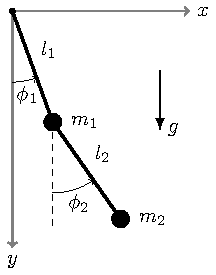
\includegraphics[page=1]{Figures/tikzpics.pdf}
\end{figure}
}
{
The generalized co-ordinates of the system are the two angles $\phi_1$ and $\phi_2$. We need to express the Cartesian co-ordinates in terms of those two angles. First, the Cartesian position of the particle $m_1$ is
\begin{align*}
    x_1 &= f_1(\phi_1) = l_1 \sin{\phi_1} \\
    y_1 &= g_1(\phi_1) = l_1 \cos{\phi_1} .
\end{align*}
By taking the time derivative of those, we obtain
\begin{align*}
    \Dot{x}_1 &= \pd{f_1}{\phi_1} \Dot{\phi}_1 = l_1 \cos{\phi_1} \Dot{\phi}_1 \\
    \Dot{y}_1 &= \pd{g_1}{\phi_1}\Dot{\phi}_1 = -l_1 \sin{\phi_1} \Dot{\phi}_1 .
\end{align*}
Substituting these expressions in the Lagrangian, we obtain the desired Lagrangian form, that is
\begin{align*}
    L_1 &= T_1 - U_1 \\
    &= \frac{1}{2} m_1 (\Dot{x}_1^2 + \Dot{y}_1^2) + m_1 g y_1 \\
    &= \frac{1}{2} m_1 l_1^2 \Dot{\phi}_1^2 + m_1 g l_1 \cos{\phi_1} . \numberthis \label{C1P1_L1}
\end{align*}
Second, the Cartesian position of the particle $m_2$ is
\begin{align*}
    x_2 &= f_2(\phi_1, \phi_2) = l_1 \sin{\phi_1} + l_2 \sin{\phi_2} \\
    y_2 &= g_2(\phi_1, \phi_2) = l_1 \cos{\phi_1} + l_2 \cos{\phi_2} .
\end{align*}
By taking the time derivative of those, we obtain
\begin{align*}
    \Dot{x}_2 &= \sum_k \pd{f_2}{\phi_k} \Dot{\phi}_k = l_1 \Dot{\phi}_1 \cos{\phi_1} + l_2 \Dot{\phi}_2 \cos{\phi_2} \\
    \Dot{y}_2 &= \sum_k \pd{g_2}{\phi_k} \Dot{\phi}_k = -l_1 \Dot{\phi}_1 \sin{\phi_1} -l_2 \Dot{\phi}_2 \sin{\phi_2} .
\end{align*}
Substituting these expressions in the Lagrangian, we obtain the desired Lagrangian form, that is
\begin{align*}
    L_2 &= T_2 - U_2 \\
    &= \frac{1}{2} m_2 (\Dot{x}_2^2 + \Dot{y}_2^2) + m_2 g y_2 \\
    &= \frac{1}{2} m_2 (l_1^2\Dot{\phi}_1^2 + l_2^2\Dot{\phi}_2^2 + 2l_1l_2\Dot{\phi}_1\Dot{\phi}_2\cos{(\phi_1 - \phi_2)}) + m_2 g (l_1 \cos{\phi_1} + l_2 \cos{\phi_2}) , \numberthis \label{C1P1_L2}
\end{align*}
where the angle difference identity as been used. Finally, the Lagrangian of the complete system is simply the sum of \eqref{C1P1_L1} and \eqref{C1P1_L2}, thus
}
{
\begin{align*}
    L = &\frac{1}{2}(m_1+m_2)l_1^2\Dot{\phi}_1^2 + \frac{1}{2}m_2l_2^2\Dot{\phi}_2^2 + m_2l_1l_2\Dot{\phi}_1\Dot{\phi}_2\cos{(\phi_1-\phi_2)} \\
    &+ (m_1+m_2)gl_1\cos{\phi_1} + m_2gl_2\cos{\phi_2}
\end{align*}
}
\end{problem}

% ============ Problem 2 ============ %

\begin{problem}
{
Find the Lagrangian of a simple pendulum of mass $m_2$, with a mass $m_1$ at the point of support which can move on a horizontal line lying in the plane in which $m_2$ moves when placed in a uniform gravitational field (acceleration $g$).
\begin{figure}[H]
    \centering
    \includegraphics[page=2]{Figures/tikzpics.pdf}
\end{figure}
}
{
The generalized co-ordinates $q$ of the system are the position $x$ and the angle $\phi$. Therefore, the Lagrangian of the first particle is simply
\begin{equation}
    L_1 = T_1 = \frac{1}{2} m_1 \Dot{x}^2. \label{C1P2_L1}
\end{equation}
The Cartesian position of the particle $m_2$ can be express in terms of the generalized co-ordinates by
\begin{align*}
    x_2 &= f_2(x, \phi) = x + l \sin{\phi} \\
    y_2 &= g_2(x, \phi) = l \cos{\phi} .
\end{align*}
The time derivative of the position is then
\begin{align*}
    \Dot{x}_2 &= \sum_k \pd{f_2}{q_k} \Dot{q}_k = \Dot{x} + l \Dot{\phi} \cos{\phi} \\
    \Dot{y}_2 &= \sum_k \pd{g_2}{q_k} \Dot{q}_k = - l \Dot{\phi} \sin{\phi} .
\end{align*}
\begin{align*}
    L_2 &= T_2 - U_2 \\
    &= \frac{1}{2} m_2 (\Dot{x}_2^2 + \Dot{y}_2^2) + m_2 g y_2 \\
    &= \frac{1}{2} m_2 (\Dot{x}^2 + l^2 \Dot{\phi}^2 + 2 l \Dot{x} \Dot{\phi} \cos{\phi}) + m_2 g l \cos{\phi} . \numberthis \label{C1P2_L2}
\end{align*}
Finally, the Lagrangian of the complete system is the sum of the two Lagrangian \eqref{C1P2_L1} and \eqref{C1P2_L2}, thus
}
{
\begin{equation*}
    L = \frac{1}{2} (m_1 + m_2) \Dot{x}^2 +  \frac{1}{2} m_2 (l^2 \Dot{\phi}^2 + 2 l \Dot{x} \Dot{\phi} \cos{\phi} ) + m_2 g l \cos{\phi}
\end{equation*}
}
\end{problem}

% ============ Problem 3 ============ %

\begin{problem} 
{
Find the Lagrangian of a simple pendulum of mass $m$, when placed in a uniform gravitational field (acceleration $g$), whose point of support ...
\begin{figure}[H]
    \centering
    \includegraphics[page=3]{Figures/tikzpics.pdf}
\end{figure}
}{}{}
\end{problem}
\begin{subproblem}
{
moves uniformly on a vertical circle with constant frequency $\gamma$.
}
{
If we set that the rotation of the point of support is counterclockwise, the Cartesian position of the particle $m$ is
\begin{align*}
    x &= f(\phi_1) = a \cos{\gamma t} + l \sin{\phi} \\
    y &= g(\phi_1) = -a \sin{\gamma t} + l \cos{\phi} .
\end{align*}
The time derivative of the position is then
\begin{align*}
    \Dot{x} &= -a \gamma \sin{\gamma t} + l \Dot{\phi} \cos{\phi} \\
    \Dot{y} &= -a \gamma \cos{\gamma t} - l \Dot{\phi} \sin{\phi} .
\end{align*}
The potential energy of the system is 
\begin{align*}
    U &= -mgy \\
    &= -mg(-a \sin{\gamma t} + l \cos{\phi}).
\end{align*}
The term $mga \sin{\gamma t}$ only depend on time and can therefore be ignored (does not contribute to the equations of motion). The kinetic energy of the particle, for its part, is
\begin{align*}
    T &= \frac{1}{2} m (\Dot{x}^2 + \Dot{y}^2)\\
    &= \frac{1}{2} m \left(l^2\Dot{\phi}^2 + a^2\gamma^2 +2a\gamma l \Dot{\phi}\sin{(\phi - \gamma t)}\right),
\end{align*}
using again the angle difference identity (I will stop mentioning it). We can observe that the term $\frac{1}{2}ma^2\gamma^2$ is a constant, thus can be ignored. The last term of the kinetic energy can also be simplified. Indeed, 
\begin{align*}
      m a\gamma l \Dot{\phi}\sin{(\phi - \gamma t)} &= m a l \gamma (\dot{\phi} - \gamma) \sin(\phi - \gamma t) + m a l \gamma^2 \sin(\gamma t - \phi) \\
     &= \frac{d}{dt} \left(-m a l  \gamma \cos(\phi - \gamma t) \right) + m a l  \gamma^2 \sin(\phi - \gamma t) .
\end{align*}
After dropping the total time derivative, we can finally get the Lagrangian
}
{
\begin{equation*}
    L = \frac{1}{2} m l^2\Dot{\phi}^2 + m a l  \gamma^2 \sin(\phi - \gamma t)  + mgl\cos{\phi}
\end{equation*}
}
\end{subproblem}

\begin{subproblem}
{
oscillates horizontally in the plane of motion of the pendulum according to the law $x=a\cos{\gamma t}$.
}
{
The Cartesian position of the particle $m$ is
\begin{align*}
    x &= f(\phi_1) = a \cos{\gamma t} + l \sin{\phi} \\
    y &= g(\phi_1) = l \cos{\phi} .
\end{align*}
The time derivative of the position is then
\begin{align*}
    \Dot{x} &= -a \gamma \sin{\gamma t} + l \Dot{\phi} \cos{\phi} \\
    \Dot{y} &= - l \Dot{\phi} \sin{\phi} .
\end{align*}
The potential energy of the system is 
\begin{equation*}
    U = -mgy = -mgl\cos{\phi},
\end{equation*}
and the kinetic energy
\begin{align*}
    T &= \frac{1}{2} m (\Dot{x}^2 + \Dot{y}^2)\\
    &= \frac{1}{2} m \left(l^2\Dot{\phi}^2 + a^2\gamma^2\sin^2{\gamma t} - 2a\gamma l \Dot{\phi}\sin{\gamma t}\cos{\phi}\right).
\end{align*}
We first see that the term $\frac{1}{2} m a^2\gamma^2\sin^2{\gamma t}$ only depend on time. The last term of the kinetic energy can also be simplified. Indeed, 
\begin{align*}
      - m a\gamma l \Dot{\phi}\sin{\gamma t}\cos{\phi} &= 
      -m l a \gamma (\gamma \cos{\gamma t} \sin{\phi} + \Dot{\phi} \sin{\gamma t}\cos{\phi}) + m l a \gamma^2 \cos{\gamma t}\sin{\phi} \\
      &= \frac{d}{dt} \left( -mla\gamma\sin{\gamma t}\sin{\phi} \right) + m l a \gamma^2 \cos{\gamma t}\sin{\phi}.
\end{align*}
After dropping the total time derivative, we can finally get the Lagrangian
}
{
\begin{equation*}
    L = \frac{1}{2} m l^2\Dot{\phi}^2 + m l a \gamma^2 \cos{\gamma t}\sin{\phi}  + mgl\cos{\phi}
\end{equation*}
}
\end{subproblem}

\begin{subproblem}
{
 oscillates vertically according to the law $y=a\cos{\gamma t}$.
}
{
The Cartesian position of the particle $m$ is
\begin{align*}
    x &= f(\phi_1) = l \sin{\phi} \\
    y &= g(\phi_1) = a \cos{\gamma t} + l \cos{\phi} .
\end{align*}
The time derivative of the position is then
\begin{align*}
    \Dot{x} &= l \Dot{\phi} \cos{\phi} \\
    \Dot{y} &= -a \gamma \sin{\gamma t} - l \Dot{\phi} \sin{\phi} .
\end{align*}
The potential energy of the system is 
\begin{equation*}
    U = -mgy = -mg \left( a \cos{\gamma t} + l \cos{\phi} \right),
\end{equation*}
The term $mga \cos{\gamma t}$ only depend on time and can therefore be ignored. The kinetic energy is
\begin{align*}
    T &= \frac{1}{2} m (\Dot{x}^2 + \Dot{y}^2)\\
    &= \frac{1}{2} m \left(l^2\Dot{\phi}^2 + a^2\gamma^2\sin^2{\gamma t} + 2a\gamma l \Dot{\phi}\sin{\gamma t}\sin{\phi}\right).
\end{align*}
We first see that the term $\frac{1}{2} m a^2\gamma^2\sin^2{\gamma t}$ only depend on time. The last term of the kinetic energy can also be simplified. Indeed, 
\begin{align*}
       m a\gamma l \Dot{\phi}\sin{\gamma t}\sin{\phi} &= 
      m l a \gamma (-\gamma \cos{\gamma t} \cos{\phi} + \Dot{\phi} \sin{\gamma t}\sin{\phi}) + m l a \gamma^2 \cos{\gamma t}\cos{\phi} \\
      &= \frac{d}{dt} \left( mla\gamma\cos{\gamma t}\sin{\phi} \right) + m l a \gamma^2 \cos{\gamma t}\cos{\phi}.
\end{align*}
After dropping the total time derivative, we can finally get the Lagrangian
}
{
\begin{equation*}
    L = \frac{1}{2} m l^2\Dot{\phi}^2 + m l a \gamma^2 \cos{\gamma t}\cos{\phi}  + mgl\cos{\phi}
\end{equation*}
}
\end{subproblem}

% ============ Problem 4 ============ %

\begin{problem}
{
Find the Lagrangian of a simple pendulum of the system below when placed in a uniform gravitational field (acceleration $g$). The particle $m_2$ moves on a vertical axis and the whole system rotates about this axis with a constant angular velocity~$\Omega$.
\begin{figure}[H]
    \centering
    \includegraphics[page=4]{Figures/tikzpics.pdf}
\end{figure}
}
{
The position of each particle $m_1$ is best described in cylindrical coordinates, which is
\begin{align*}
    r_1 &= a \sin{\theta} \\
    \phi_1 &= \phi \\
    z_1 &= a \cos{\theta},
\end{align*}
where $\phi$ is the angle of rotation of the system about the axis; $\Dot{\phi} = \Omega$. The kinetic energy of each particle $m_1$ is thus
\begin{align*}
    T_1 &= \frac{1}{2} m_1 ( \Dot{r}_1^2 + r_1^2\Dot{\phi}_1^2 + \Dot{z}_1^2 ) \\
    &= \frac{1}{2} m_1 ( a^2\Dot{\theta}^2\cos^2{\theta} + a^2\Omega^2\sin^2{\theta} + a^2\Dot{\theta}^2\sin^2{\theta} ) \\
    &= \frac{1}{2} m_1 a^2 ( \Dot{\theta}^2 + \Omega^2\sin^2{\theta} ) . \numberthis \label{C1P4_T1}
\end{align*}
The potential energy of this particle can be found by using the $z$ component of his position, namely
\begin{align*}
    V_1 &= -m_1gz_1 \\
    &= -m_1ga\cos{\theta}. \numberthis \label{C1P4_V1}
\end{align*}
The particle $m_2$, in its case, can only move up and down, thus its position can be completely defined by
\begin{equation*}
    z_2 = 2 a \cos{\theta}.
\end{equation*}
Then, the kinetic energy of each particle $m_2$ is
\begin{align*}
    T_2 &= \frac{1}{2} m_2 \Dot{z}_2^2 \\
    &= m_2 a^2 \Dot{\theta}^2 \sin^2{\theta} \numberthis \label{C1P4_T2}
\end{align*}
and the potential energy is
\begin{align*}
    V_2 &= - m_2 g z_2 \\
    &= - 2 m_2 g a \cos{\theta}. \numberthis \label{C1P4_V2}
\end{align*}
Using \eqref{C1P4_T1}, \eqref{C1P4_V1}, \eqref{C1P4_T2} and \eqref{C1P4_V2}, the Lagrangian of the system is
\begin{equation*}
    L = 2(T_1 + T_2 - V_1 - V_2),
\end{equation*}
therefore
}
{
\begin{equation*}
    L = m_1 a^2 ( \Dot{\theta}^2 + \Omega^2\sin^2{\theta} ) + 2m_2 a^2 \Dot{\theta}^2 \sin^2{\theta} + 2(m_1+2m_2)ga\cos{\theta}
\end{equation*}
}
\end{problem}